\documentclass{beamer}

\usepackage{ucs}
\usepackage[utf8x]{inputenc}
\usepackage[T1]{fontenc}
\usepackage[english]{babel}
\usepackage{epstopdf}
\usepackage{algpseudocode}
%\usepackage{algorithmicx}
\usepackage{algorithm}

\usepackage{subfig}
\usepackage{algpseudocode}
\usepackage{algorithmicx}
\usepackage{algorithm}
\usepackage{relsize}%	relative font sizes
\usepackage{multicol}
\usepackage{multirow}
\usepackage{todonotes}
\usepackage{xspace}

\usepackage{todonotes}
\presetkeys{todonotes}{inline}{}
%\newcommand{\todoline}[2][inline]{\todo[#1]{#2}}

\newcommand{\todopfac}[1]{\todo[color=red!40]{#1}}
\newcommand{\todonaps}[1]{\todo[color=green!40]{#1}}

\graphicspath{{../images/}}

\newsavebox{\ieeealgbox}
\newenvironment{alg}
  {
   \begin{lrbox}{\ieeealgbox}
   \begin{minipage}{\dimexpr\columnwidth-2\fboxsep-2\fboxrule}
   \hrulefill
   \begin{algorithmic}
  }
  {
   \end{algorithmic}
   \hrulefill
   \end{minipage}\end{lrbox}\noindent\mbox{\usebox{\ieeealgbox}}
  }

% Title page

%\title{TreeTiler Optimization Techniques applied to the Galois System}
\title[Improving Locality]{Improving Locality on Traversal of Recursive Structures}

\author[M. Palhas \and P. Costa]{Miguel~Palhas \and Pedro~Costa}
%\smaller Stéphane Clain (co-Advisor)\\
% Andrew
% Donald

\date{Austin, Texas, U.S.A. --- August 2012}

\subject{Summer Internship}



\institute[ICES @ UTexas]{
	Institute for Computational Engineering and Sciences\\
	University of Texas
}

\date{Braga, June 2012}


%	beamer options
\usetheme{CambridgeUS}

\begin{document} %	begin presentation

\frame[plain]{\titlepage}

\frame{\frametitle{Index}\tableofcontents}

% TreeTiler (the paper)
\section{TreeTiler}
% TODO da minha parte esta feito

\frame{
	\frametitle{TreeTiler}

	\begin{itemize}\itemsep=20pt
		\item Transformation Framework proposed by Milind Kulkarni and Yougjoon Jo on \textit{``Enchancing Locality for Recursive Traversals of Recursive Structures''};
		
		\item Uses JastAdd to refactor Java code at compile time;

		\item Automatically identifies recursive structures, and applies optimizations to how the traversal is done, to exploit locality;

		\item AutoTuner to determine optimal parameters:
		\begin{itemize}
			\item Parameters are dependent of hardware, algorithm and input;
			% NOTE: machine details:   cache size
			% NOTE: algorithm details: optimal block size for barnes-hut is different than for ray tracer
			% NOTE: input dependency:  ray tracer with too few spheres will not benefit from blocking at all
			\item Sampling at runtime to find best parameters;
		\end{itemize}
	\end{itemize}
}

  \subsection{Optimization Techniques}
  \frame{
	\frametitle{Spatial Sort}
	%\todonaps{Spatial Sort}

	\begin{columns}
		\column{.7\textwidth}
			\begin{itemize}\itemsep=20pt
				\item Points closer in space are more likely to follow a similar traversal

				\item By sorting items, this can be exploited for locality
			\end{itemize}

		\column{0.3\textwidth}
		TEXT
	\end{columns}

	\textbf{Fails when traversal depth is too large to fit in cache}
}
  \frame{
	\frametitle{Blocking}

		\begin{columns}
		\column{.6\textwidth}
			\begin{itemize}\itemsep=20pt
				\item Grouping traversals in blocks allows locality improvements for deeper structures

				\item All block elements must follow similar path (achieved with Spatial Sort)
			\end{itemize}
		
			\begin{figure}
				\centering
				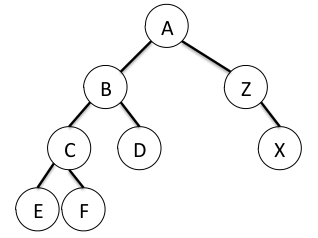
\includegraphics[width=0.5\columnwidth]{pointblocking_tree}
			\end{figure}

		\column{0.4\textwidth}

			\begin{figure}
				\centering
				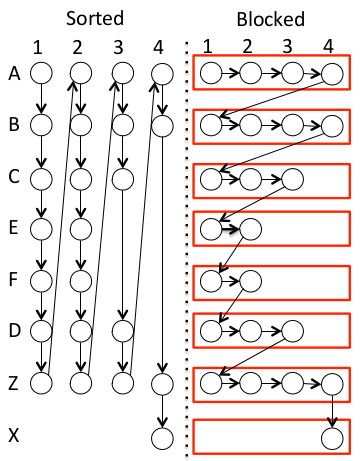
\includegraphics[width=0.9\columnwidth]{pointblocking_blocks}
			\end{figure}
	\end{columns}
}
  % \frame{%
\frametitle{Auto Tuning}%
\todonaps{Auto Tuning}%
}

\section{Case Studies}
\frame{
	\frametitle{Case Studies}

	Studied optimizations applied to three different test cases:
	\begin{itemize}\itemsep=15pt
		\item Barnes-Hut
		\begin{itemize}
			\item[-] N-Body
			\item[-] Octree
		\end{itemize}

		\item Two Point Correlation
		\begin{itemize}
			\item[-] N-Body
			\item[-] kD-Tree
		\end{itemize}

		\item Path Tracing
		\begin{itemize}
			\item[-] Ray Tracing algorithm
			\item[-] Bounding Volume Hierarchy
		\end{itemize}
	\end{itemize}
}

  \subsection{Barnes-Hut}
  \begin{frame}
	\frametitle{Barnes-Hut}
	\vfill
	\begin{description}
		\item[Type:] N-Body problem;
		\item[Domain:] Bodies in space;
		\item[Goal:] Compute the evolution of a system of particles in time;
	\end{description}
	\vfill
	\begin{block}{Acceleration Structure}
		\begin{itemize}
			\item Octree;
			\item If a given cell is too far away, the cell itself is used to calculate interactions;
		\end{itemize}
	\end{block}
	\vfill
\end{frame}

\begin{frame}
	\frametitle{Strategy}
	\begin{itemize}\itemsep=20pt
		\item Change in the tree traversal:
		\begin{itemize}
			\item[-] \textbf{Original approach}: The tree is analysed from the root for each body;
			\item[-] \textbf{New approach}: The tree is analysed for a block of points at a time;
		\end{itemize}
		\item Spatial Sort the bodies by coordinates;
		\item Optimization only applied to the computation of the forces.
	\end{itemize}
\end{frame}

\begin{frame}
	\frametitle{Expectations}
	\begin{itemize}\itemsep=20pt
		\item For deep structures, sorting is unlikely to improve results;
		\item Point blocking is expected to lower considerably cache misses;
		\item Original work achieved improvements around 70\%;
	\end{itemize}
\end{frame}

  \subsection{Two Point Correlation}
  \frame{
	\frametitle{Two Point Correlation}
	\todonaps{Two Point Correlation}
}
  \subsection{Ray Tracer}
  \frame{
	\frametitle{Ray Tracer}
	
	\begin{block}{}
		\begin{itemize}
			\item Simple Monte Carlo Path Tracer

			\item Based on \texttt{smallpt}: \textit{Global Illumination in 99 lines of C++}
		\end{itemize}
	\end{block}

	\begin{block}{Workflow}
		\begin{itemize}\itemsep=15pt
			\item Each pixel generates $N$ rays
			\begin{itemize}
				\item[-] $N > 10^4$
			\end{itemize}

			\item Each ray generates new sub-rays

			\item Bounding Volume Hierarchy for the scene
		\end{itemize}
	\end{block}
}

%
% Strategy
%
\frame{
	\frametitle{Ray Tracer}

	\begin{block}{Strategy}
		\begin{enumerate}\itemsep=15pt

			\item Change iteration method
			\begin{itemize}
				\item[-] \textbf{Original approach}: Distribute pixels accross threads
				\item[-] \textbf{New approach}: One pixel at a time. Distribute rays
				% NOTE: there are enough rays for this
				% NOTE: original was using OpenMP
			\end{itemize}
			
			\item Spatial Sort all rays by ray origin

			\item Spatial Sort on each block by ray direction

			\item Each ray updates itself, and keeps track of current contribution

			\item Reduction to compute final pixel color
		\end{enumerate}
	\end{block}
}

%
% Expectations
%
\frame{
	\frametitle{Ray Tracer}

	\begin{block}{Expectations}
		\begin{itemize}\itemsep=15pt

			\item Ray Tracer required more data per item, and more auxiliary data during traversal

			\item Ray Blocking can only be useful for more complex scenes. But that also increases ray divergence

			\item Spatial Sort is not enough to keep coherence between rays.
			\begin{itemize}
				\item Other strategies solve this more effectively (e.g. Coherent Path Tracing)
			\end{itemize}

			\item Original work presents Ray Tracer as the worst test case (max speedups around 10\%)
			
		\end{itemize}
	\end{block}
}

\section{Results}
\frame{
	\frametitle{Results}
	\todonaps{Results}
	\textbf{Y U NO SPEEDUP?!}
}

\section{Conclusions}
\begin{frame}
	\frametitle{Conclusions}
	\begin{itemize}\itemsep=15pt
		\item Spatial Sort is relevant when traversing a recursive structure;
		\begin{itemize}
			\item For smaller traversals, it is enough to gain locality.
		\end{itemize}

		\item With larger traversals, Point Blocking also proves useful;
		%takes advantage of sorting by grouping the objects during the traversal;

		\item Ray tracer limited by larger memory footprint and incoherence;

		\item Results show improvements:
		\begin{table}
			\begin{tabular}{|c|cc|}
				\hline
				& \textbf{Speedup} & \textbf{Misses Decrease}	\\
				\hline
				\textbf{Barnes-hut} &  1.48 & 93\%	\\
				\textbf{Point Correlation} & 1.54 & 98\%	\\
				\textbf{Ray Trace} & 0.77 & 44\%	\\
				\hline
			\end{tabular}
		\end{table}
	\end{itemize}
\end{frame}

% Case Studies:
%    Barnes-hut
%    Point correlation
%    Ray Tracer - explain why its not an effective technique here
%
% Results.dump()

\begin{frame}[plain]
	\titlepage
	\begin{center}
		\Huge\bfseries - ? -
	\end{center}
\end{frame}

\end{document}%	end presentation
